%versi 2 (8-10-2016) 
\chapter{Pendahuluan}
\label{chap:intro}
   
\section{Latar Belakang}
\label{sec:latarbelakang}

Kemajuan teknologi memudahkan manusia untuk mencari berbagai macam informasi. Salah satu informasi yang dapat diperoleh adalah informasi tentang navigasi transportasi publik. KIRI  adalah perangkat lunak yang berguna sebagai navigasi antar kota menggunakan transportasi publik dengan menggunakan perangkat peta digital\cite{pascal:17:KIRI}. Pada awal pembuatannya KIRI dibuat untuk tujuan komersial. Namun karena dinilai kurang sukses, projek KIRI sekarang menjadi open source projek yang dapat di akses. Bentuk tampilan aplikasi KIRI dapat dilihat pada gambar \ref{fig:kiri}.

\begin{figure}[H]
	\centering
	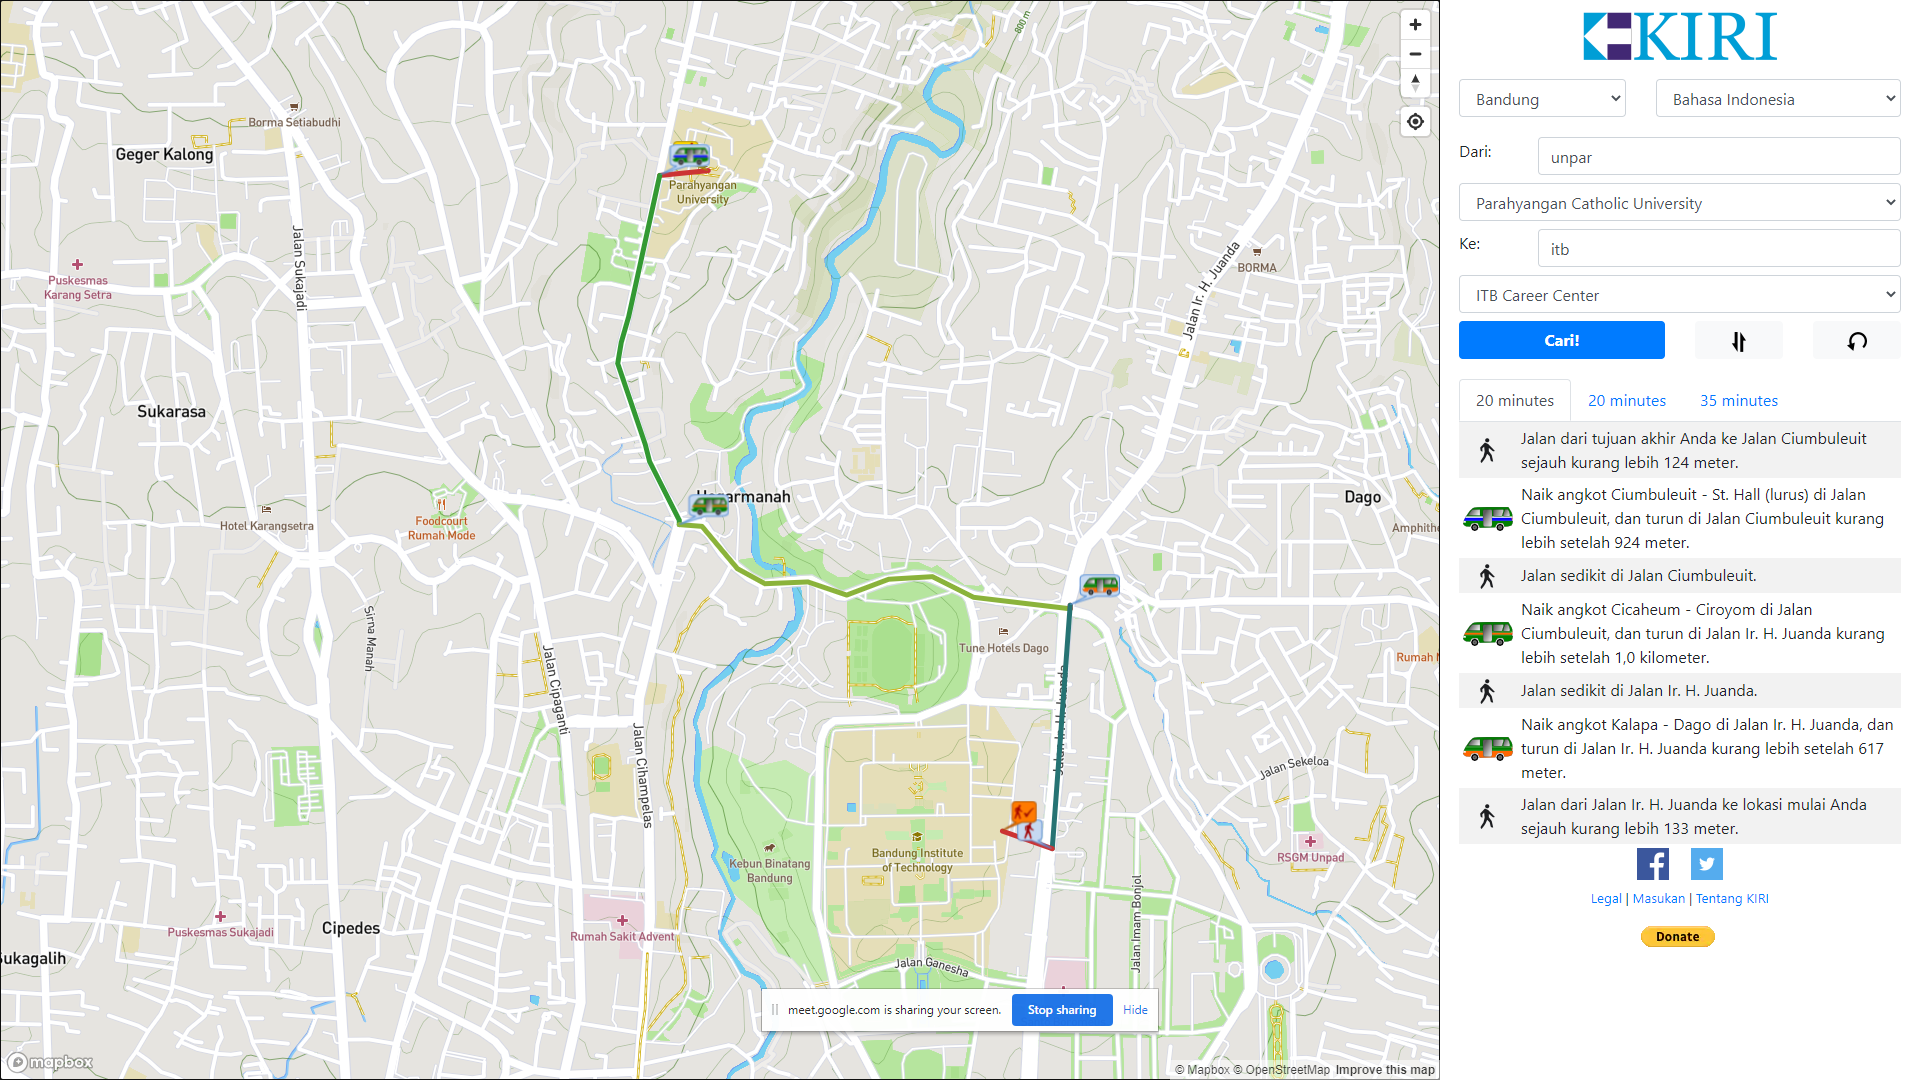
\includegraphics[scale=0.3]{Gambar/kiri-example-1.png}
	\caption{Tampilan Utama Website KIRI}
	\label{fig:kiri}
\end{figure}

Pada perangkat lunak KIRI seluruh aktivitas yang dilakukan oleh user sudah tercatat. Data yang tercatat disebut juga dengan data histori. Data histori kiri memiliki jumlah record yang cukup banyak sehingga memungkinkan untuk mendapatkan informasi dari data tersebut. Tetapi data histori tersebut belum diolah secara maksimal.

Visualisasi Data adalah teknik  untuk mengkomunikasikan data atau informasi dengan menggunakan objek visual  seperti \textit{graphic, chart, diagram, dll}. Salah satu objek visual yang dapat digunakan untuk merepresentasikan data adalah \textit{Google Maps}.

Metode yang akan digunakan dalam memvisualisasikan data adalah \textit{Heat Map} dan \textit{Marker Clustering}. \textit{Heat Map} adalah teknik visualisasi data yang menunjukkan besarnya suatu fenomena sebagai warna dalam dua dimensi. Sedangkan \textit{Marker Clustering}  adalah teknik visualisasi data  yang  mengelompokan \textit{marker} atau \textit{pointer} yang jarak \textit{latitude} dan \textit{longitude} nya saling berdekatan antara suatu \textit{marker} dengan marker yang lainnya. Contoh bentuk \textit{heat map} dan \textit{marker clustering} dapat dilihat pada gambar \ref{fig:hm} dan \ref{fig:mc}
\begin{figure}[H]
	\centering
	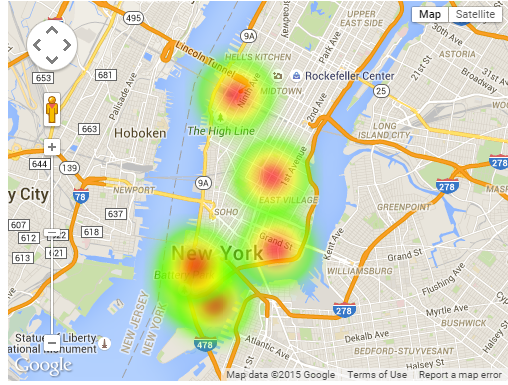
\includegraphics[scale=0.5]{Gambar/heat-map-example.png}
	\caption{Tampilan Heat Map}
	\label{fig:hm}
\end{figure}

\begin{figure}[H]
	\centering
	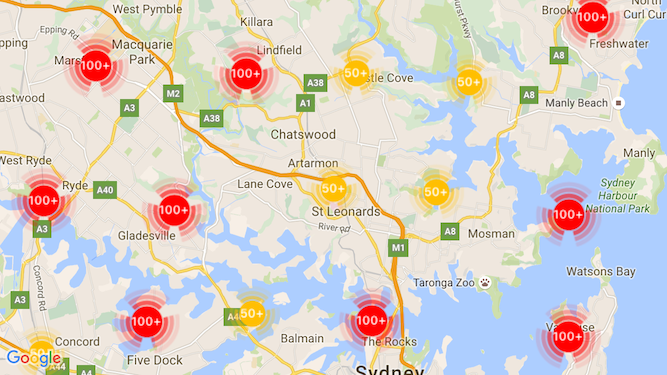
\includegraphics[scale=0.3]{Gambar/markerclustering.PNG}
	\caption{Tampilan Marker Clustering}
	\label{fig:mc}
\end{figure}

Pada skripsi ini akan dibangun perangkat lunak yang dapat memvisualisasikan data histori KIRI. Perangkat lunak ini akan menggunakan metode visualisasi \textit{heat map} dan \textit{marker clustering} dari hasil visualisasi tersebut akan diambil suatu pola kesimpulan dari data histori KIRI.


\section{Rumusan Masalah}
\label{sec:rumusan}
Rumusan masalah dari topik ini adalah sebagai berikut:
\begin{itemize}
  \item Bagaimana memvisualisasikan data histori KIRI?
  \item Bagaimana menemukan pola dari data histori KIRI?
  \item Bagaimana penerapan metode \textit{heat map} pada visualisasi data histori KIRI?
  \item Bagaimana penerapan metode \textit{marker clustering} pada visualisasi data histori KIRI?
\end{itemize}

\section{Tujuan}
\label{sec:tujuan}
Tujuan dari topik ini adalah sebagai berikut:
\begin{itemize}
  \item Menggunakan \textit{Google Maps Javascript API}.
  \item Melakukan pengujian menggunakan metode observasi.
  \item Mengimplementasikan metode \textit{Heat map} pada visualisasi data histori KIRI.
  \item Mengimplementasikan metode \textit{Marker clustering} pada visualisasi data histori KIRI.
\end{itemize}

\section{Batasan Masalah}
\label{sec:batasan}
Penelitian ini dibuat dengan batasan - batasan berikut:
\begin{enumerate}
	\item Perangkat lunak ini hanya akan menampilkan data pada daerah Bandung saja.
\end{enumerate}


\section{Metodologi}
\label{sec:metlit}
Metodologi yang digunakan dalam penelitian ini adalah:
	\begin{enumerate}
		\item Mempelajari \textit{Google Maps Javascript API} khususnya \textit{Heat Map} dan \textit{Marker Clustering}.
		\item Analisis  perangkat lunak yang akan dibangun.
		\item Merancang perangkat lunak yang akan dibangun.
		\item Membangun perangkat lunak yang mengimplementasikan \textit{Heat Map} atau \textit{Marker Clustering} dengan memanfaatkan \textit{Google Maps Javascript API}.
		\item Menentukan pola dari hasil visualisasi data.
		\item Analisis hasil pengujian dan mengambil kesimpulan.
	\end{enumerate}


\section{Sistematika Pembahasan}
\label{sec:sispem}
Laporan penelitian tersusun ke dalam enam bab secara sistematis sebagai berikut.
\begin{itemize}
    \item Bab 1 Pendahuluan\\
    Berisi latar belakang, rumusan masalah, tujuan, batasan masalah, metodologi penelitian, dan sistematika pembahasan.
   
   \item Bab 2 Dasar Teori\\
    Berisi  metode penentuan pola, \textit{library Google Maps} dan bahasa pemograman \textit{Javascript}
   
    \item Bab 3 Analisis\\
    Berisi analisis masalah terkait implementasi \textit{Goole Map}, studi kasus teknik penentuan pola yang diimplementasikan, dan gambaran umum perangkat lunak yang meliputi diagram aktivitas dan diagram kelas.
  
    \item Bab 4 Perancangan Perangkat Lunak\\
    Berisi perancangan perangkat lunak yang akan dibangun, meliputi perancangan antarmuka,
diagram kelas lengkap dan masukan perangkat lunak.
    
    \item Bab 5 Implementasi dan Pengujian\\
Berisi implementasi antarmuka perangkat lunak, pengujian fungsional, pengujian eksperimental
serta kesimpulan dari pengujian.
   
    \item Bab 6 Kesimpulan dan Saran\\
    Berisi kesimpulan dari awal hingga akhir penelitian dan saran untuk penelitian berikutnya.
\end{itemize}